% \documentclass[12pt,openright,oneside,a4paper,brazil]{abntex2}
% \usepackage[utf8]{inputenc}
% \counterwithout{section}{section}
% \counterwithout{figure}{chapter}
% \counterwithout{table}{chapter}
% \setlength{\parindent}{1.3cm}
% \usepackage{indentfirst}
% \setlength{\parskip}{0.2cm}
% \usepackage[bottom=2cm,top=3cm,left=3cm,right=2cm]{geometry}
% \usepackage{graphicx}
% \graphicspath{{figuras/}}
% \usepackage{placeins}
% \usepackage{longtable}
 
 %opening
% \title{}
% \author{}
 
%\begin{document}
 
 
 \textual
\begin{center}
 {\large Documento de visão técnica}\\[0.2cm]
 \end{center}


\section*{Introdução}
Como tentativa de amenizar os problemas gerados pela falta de água potável na cidade de Acarí - RN, foi proposto um sistema capaz de gerar água de boa qualidade a partir da umidade do ar. Para o correto funcionamento desse sistema é necessário um software capaz de permitir o monitoramento da água.

O objetivo primário do software proposto será o monitoramento da qualidade e disponibilidade da água. Além disso, ele disponibilizará outras informações relacionadas a tecnologia proposta referentes, por exemplo, à turbina, à casa de controle, ao monitoramento da adição de sais.

\section*{Descrição do Problema}
Encontra-se abaixo tabelas com as descrições dos problemas identificados:
\begin{table}[!h]
\centering
\begin{tabular}{|p{4cm}|p{10cm}|}\hline
\textbf{O problema de:}&Falta de um software para monitorar o funcionamento da tecnologia projetada.\\ \hline
\textbf{Que afeta:}&A qualidade da tecnologia proposta.\\ \hline
\textbf{Cujo o Impacto é:}&	O mau funcionamento do sistema de obtenção de água, e a não garantia de distribuição de água potável.\\ \hline
\textbf{Uma solução seria:}&	A implementação de um software para o monitoramento do sistema como um todo.\\ \hline

\end{tabular}
\end{table}

\begin{table}[!h]
\centering
\begin{tabular}{|p{4cm}|p{10cm}|}\hline
\textbf{O problema de:}&Falta de informações referentes à qualidade da água.\\ \hline
\textbf{Que afeta:}&Cidadãos da cidade de Acarí - RN localizada no Rio Grande do Norte mais especificamente no bairro Vereador Tarcísio Bezerra Galvão.\\ \hline
\textbf{Cujo o Impacto é:}&A não garantia da água está potável, podendo causar problemas à saúde humana.\\ \hline
\textbf{Uma solução seria:}&	A implementação de um software para a gestão do controle e qualidade da água.\\ \hline
\end{tabular}
\end{table}

\section*{Descrições dos envolvidos e usuários}
Os \emph{stakeholders} envolvidos no projeto de software são a equipe de desenvolvimento do projeto, mais diretamente a equipe formada pelos integrantes da engenharia de software, os professores da disciplina, os técnicos que serão usuários do sistema, a população que se beneficia do sistema.

\subsection*{Resumo dos Envolvidos}
A equipe composta por 27 alunos do grupo 1 da disciplina Projeto Integrador I da Universidade de Brasília, Campus Gama no 1º semestre de 2015, técnicos que ficarão responsáveis pelo acompanhamento do sistema, os professores orientadores e da população da cidade de Acarí – RN, mais especificamente no bairro Vereador Tarcísio Bezerra Galvão.

\subsection*{Resumo dos Usuários}
Os técnicos responsáveis pelo acompanhamento do sistema, irão monitorar os dados referentes a qualidade da água que serão gerados pelo sistema.

\subsection*{Ambiente do Usuários}
O sistema será implantado na casa  de Controle da planta de abastecimento da água. Esta casa de controle objetiva manter que toda o sistema esteja funcionando da maneira esperada.

\subsection*{Ambiente das Principais Necessidades dos Envolvidos ou Usuários}
A equipe deve assegurar que a água extraída pela planta esteja em um nível considerável para consumo. Caso não esteja problema causador deve ser mitigado, evitando que ocorra novamente. O técnico também abastecerá o reservatório de sais utilizados na mistura com a água caso esteja com uma pequena quantidade.

\section*{Visão geral do produto}
\subsection*{Perspectiva do Produto}
Esse software é um componente do sistema proposto de geração de água potável a partir da umidade do ar. A sua finalidade principal é o monitoramento do sistema como um todo. Nele haverá informações relacionadas à qualidade e quantidade da água obtida, características do ambiente externo onde as turbinas se encontram, casa de controle, distribuição de energia excedida, ao armazenamento e tratamento com sais da água, dados sobre a turbina. 

	Alguns dos dados referentes a turbina que serão monitorados pelo software são: as temperaturas internas, a quantidade de energia gerada por cada turbina, a velocidade de rotação das pás. A qualidade da água também será monitorada, será analisada, por exemplo, a quantidade de sais na água, o PH, a quantidade de oxigênio.
	
	Dados relacionados à casa de controle incluem, por exemplo, a voltagem das baterias, a falta ou presença de energia. Com relação a distribuição de energia, o software deve mostrar se a energia excedida está sendo direcionada a rede ou se está abastecendo a casa de controle. Também serão obtidos dados referentes a umidade do ar e as características do vento de onde as turbinas se encontram, como exemplo de dados relacionados ao ambiente externo.
	
	Percebe-se, portanto, que o software proposto visa, basicamente, possibilitar o monitoramento de uma série de aspectos relacionados a tecnologia de captação de água a partir da umidade do ar.

\subsection*{Suposições e Dependências}
É possível que haja alterações futuras no software proposto, principalmente, relacionadas a integração com eletrônica. Alterações nos componentes eletrônicos afetam diretamente o software proposto.

\section*{Recursos do produto}
Este item traz todos os recursos referentes ao produto: Os requisitos funcionais, os não funcionais e as restrições referentes ao sistema. Cada um desses requisitos possui um código de identificação para facilitar a rastreabilidade, a sua descrição e o seu nível de prioridade que são prioridade alta, média ou baixa e abaixo está estabelecido o significado de cada uma destas prioridades.
\begin{itemize}
\item Alta:  O sistema só funcionará de maneira eficaz caso este requisito esteja sendo atendido.
\item Média: O sistema pode 	funcionar caso este requisito não seja atendido.	
\item Baixa: O sistema funcionará 	normalmente caso este requisito não seja atendido.
\end{itemize}

\subsection*{Requisitos Funcionais}
%\begin{table}[!t]
%\centering
\begin{longtable}{|p{4cm}|p{9cm}|p{2cm}|}\hline	
\textbf{Código}	& \textbf{Descrição} & \textbf{Prioridade}\\ \hline	
RF1	& O sistema deve mostrar para o usuário os dados referentes a condutividade da água.	& Alta\\ \hline
RF2	& O sistema deve salvar em um log os dados recebidos pelo sensor de condutividade elétrica.	& Alta\\ \hline
RF3	& O sistema deve mostrar para o usuário os dados referentes a quantidade de oxigênio dissolvido na água.	& Alta\\ \hline
RF4	& O sistema deve salvar em um log os dados recebidos pelo sensor de oxigênio.	& Alta\\ \hline
RF5	& O sistema deve mostrar para o usuário os dados referentes a turbidez da água.	& Alta\\ \hline
RF6	& O sistema deve salvar em um log os dados recebidos pelo sensor de turbidez da água.	& Alta\\ \hline
RF7	& O sistema deve mostrar para o usuário os dados referentes ao PH da água.	& Alta\\ \hline
RF8	& O sistema deve salvar em um log os dados recebidos pelo sensor de PH da água.& 	Alta\\ \hline
RF9	& O sistema deve mostrar para o usuário os dados referentes a quantidade de nitrogênio  da água.	& Alta\\ \hline
RF10 & 	O sistema deve salvar em um log os dados recebidos pelo sensor de nitrogênio.& 	Alta\\ \hline
RF11	& Os dados de controle da água devem ser atualizados em tempo real.			& Média\\ \hline
RF12	& O sistema deve exibir gráficos com informações referentes aos dados de qualidade da água.		& Média\\ \hline
RF13& 	O sistema deve emitir um alerta caso o parâmetro de qualidade da água não esteja aceitável.& 	Alta\\ \hline
RF14	& O sistema deve permitir a consulta dos dados armazenados.			& Alta\\ \hline
RF15& 	O sistema deve permitir a consulta da quantidade da água em litros disponível no reservatório.	& Alta\\ \hline
RF16& 	O sistema deve possuir uma página de login para o acesso.		& Média	\\ \hline
RF17& 	O sistema deve possuir um mecanismo para impressão dos dados.	& Baixa\\ \hline
RF18& 	O sistema deve possuir um mecanismo para exportação dos dados.& 	Baixa		\\ \hline	
RF19& 	O sistema deve mostrar para o usuário os dados relacionados a temperatura interna da turbina no compartimento do gerador, obtidos por um sensor de temperatura.& 	Alta\\ \hline
RF20& 	O sistema deve salvar em um log os dados recebidos relacionados a temperatura interna no compartimento do gerador da turbina.	& Alta\\ \hline
RF21& 	O sistema deve mostrar para o usuário os dados relacionados a temperatura interna da turbina no compartimento do condensador, obtidos por um sensor de temperatura.	& Alta\\ \hline
RF22& 	O sistema deve salvar em um log os dados recebidos relacionados a temperatura interna no compartimento do condensador da turbina.	& Alta\\ \hline
RF23& 	O sistema deve permitir o monitoramento da velocidade e direção do ar na região onde as turbinas estão localizadas.& 	Alta\\ \hline
RF24& 	O sistema deve salvar em um log os dados recebidos relacionados ao vento obtidos pelo anemômetro.	& Média\\ \hline
RF25& 	O sistema deve permitir o monitoramento da velocidade de rotação das pás.& 	Alta\\ \hline
RF26& 	O sistema deve salvar em um log os dados recebidos relacionados a rotação das pás da turbina.	& Média\\ \hline
RF27& 	O sistema permitir o monitoramento da vibração da turbina.	& Alta\\ \hline
RF28& 	O sistema deve salvar em um log os dados recebidos relacionados a vibração da turbina.& 	Média\\ \hline
RF29& 	O sistema deve permitir o monitoramento da quantidade de energia gerada por cada turbina.	& Alta\\ \hline
RF30& 	O sistema deve permitir o monitoramento da quantidade de energia consumida pelos equipamentos presentes em cada turbina.	& Alta\\ \hline
RF31& 	O sistema deve permitir o monitoramento da quantidade de energia gerada por cada turbina.	& Alta\\ \hline
RF32& 	O sistema deve identificar se a energia está sendo direcionada à rede ou a casa de controle.	& Alta\\ \hline
RF33& 	O sistema deve permitir o monitoramento a umidade do ar do local onde a turbina se encontra. 	& Alta\\ \hline
RF34& 	O sistema deve permitir o monitoramento da quantidade de água, em litros, disponibilizada a cada dia para a população.& 	Alta\\ \hline
RF35& 	O sistema deve permitir o monitoramento da quantidade de água de baixa qualidade utilizada para finalidades alternativas.& 	Alta\\ \hline
RF36& 	O sistema deve permitir o monitoramento do nível da água presente nos reservatórios internos à turbina.	& Alta\\ \hline
RF37& 	O sistema deve permitir o monitoramento da voltagem das baterias utilizadas no sistema.	& Alta\\ \hline

\end{longtable}
%\end{table}

\subsection*{Requisitos Não Funcionais}
\textbf{Usabilidade:}O sistema deve obedecer às metas de usabilidade. Além disso, ele deve possuir um sistema de ajuda para responder eventuais duvidas do usuário.

\textbf{Confiabilidade:} O sistema deverá estar disponível 24h por dia. Além disso, o sistema não deve ser tolerante em falhas relacionados aos critérios de qualidade da água.

\textbf{Desempenho:} Todas as funcionalidades do sistema devem ser executadas em menos de 2 segundos.

\textbf{Portabilidade:} O sistema será executado no sistema operacional Windows XP ou superior. Além disso, deve existir padrões na codificação, o que ajudará em futuras manutenções.

\textbf{Linguagem:} O sistema será desenvolvido em C\#/C++.

\subsection*{Restrições do Sistema}
\begin{table}[!htp]
\centering
\begin{tabular}{|p{4cm}|p{10cm}|}\hline
\textbf{Código:}&\textbf{Descrição}\\ \hline
RS1	&O sistema operacional a ser utilizado deverá ser o Windows XP ou superior.\\ \hline
RS2	&O sistema deverá estar associado a um banco de dados local, onde ficarão armazenados os dados obtidos.\\ \hline
RS3	&O software deverá funcionar continuamente, sem interrupções.\\ \hline
RS4	&O software deve ser desenvolvido deverá ser desenvolvido na linguagem C\# ou C++.\\ \hline
RS5	&O sistema deve ser capaz de interagir com os microprocessadores definidos.\\ \hline
\end{tabular}
\end{table}

\subsection*{Modelo de Caso de Uso}
\FloatBarrier
\begin{figure}[!ht]
\centering
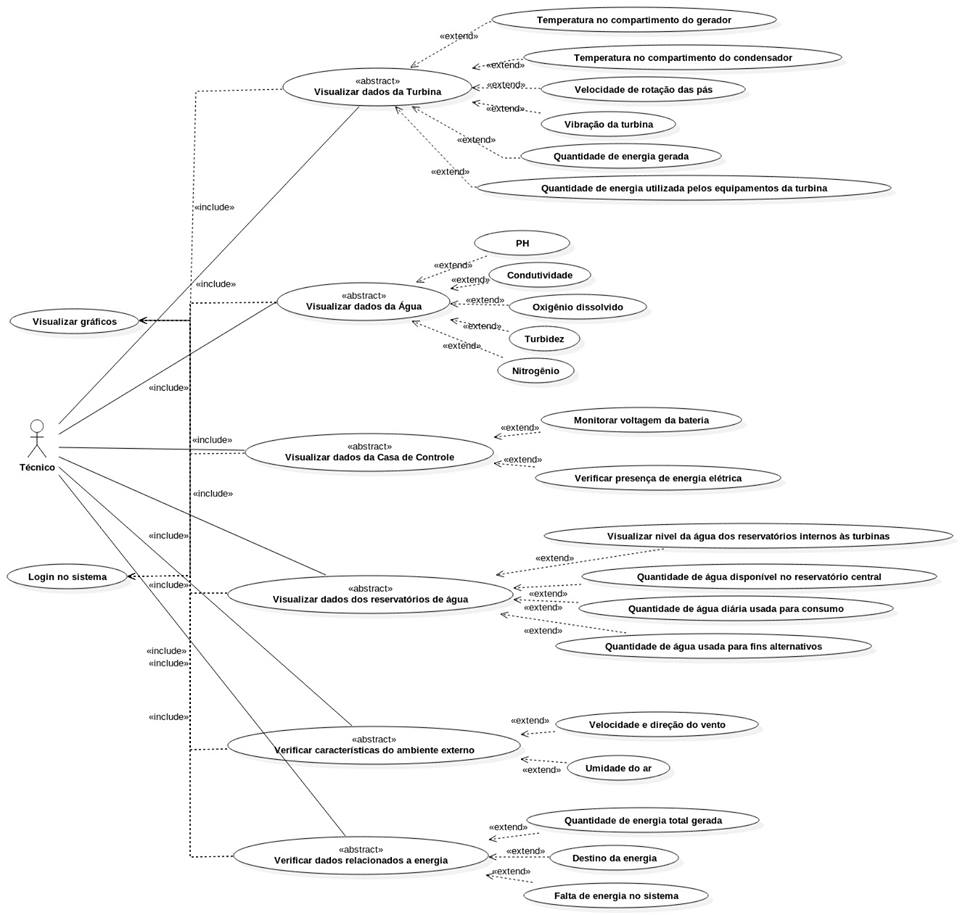
\includegraphics[scale=0.5]{figuras/modelo_caso_uso}
\caption[Modelo Caso Uso]{Modelo de caso de uso do sistema}
\label{caso_uso}
\end{figure}
\FloatBarrier
%\end{document}